---
title:
- Approximation algorithms for ground state energies of multi-qutrit systems
author:
- Luca Göcke
theme:
- Frankfurt
fonttheme:
- serif
header-includes: |
	\usepackage{braket}
	\usepackage{dsfont}
	\usepackage{bm}
	\newtheorem{lma}{Lemma}
	\newtheorem{thm}{Theorem}
---


# Outline

+ Approximation algorithms for quantum many-body systems

+ Implementation of specific models

+ Generalization to qutrits


# Approximation algorithms for quantum many-body systems

\begin{center}
Find product state approximaiton to maximal (minimal) eigenvalue of traceless $2$-local Hamiltonians $H = H_1+H_2$ where
\begin{equation}\label{ham}
	H_1 = \sum_{j=1}^{3n} D_jP_j,\quad ~ H_2  = \sum_{i,j=1}^{3n} C_{i,j}P_iP_j
\end{equation}
with the Pauli-operators $P_{3a-2}=X_a, ~ P_{3a-1}=Y_a, ~ P_{3a}=Z_a$
\end{center}


# Approximation algorithms for quantum many-body systems

\begin{thm}\emph{
		There is an efficient classical algorithm which, given $H$ of the form \eqref{ham}, outputs a product state $\ket{\phi} = \ket{\phi_1}\otimes\ldots\otimes \ket{\phi_n}$ such that with probability at least $\frac{2}{3}$
			$$\bra{\phi}H\ket{\phi}\ge \frac{\lambda_{max}(H)}{O(\log{}n)}.$$
Moreover, each single-qubit state $\phi_i$ in an eigenstate of one of the Pauli operators $X$, $Y$ or $Z$.
}\end{thm}

<!---
 # Approximation algorithms for quantum many-body systems
 + $H'=H_2+Z_{n+1}H_1$
 \begin{lma}
 	\emph{$\lambda_{max}\left( H' \right) =\lambda_{max}\left( H \right)$. Moreover, given any $(n+1)$-qubit state  $\omega$ we can efficiently compute an $n$-qubit state $\phi$ such that $$ \bra{\phi}H\ket{\phi} \ge \bra{\omega}H'\ket{\omega}.$$
 If $\omega$ is a tensor product of single qubit stabilizer states then so is $\phi$.}
 \end{lma}

 # Approximation algorithms for quantum many-body systems

 + $H'=H_2+Z_{n+1}H_1$

 + Since $H_1$ and $Z_{n+1}$ commute, they share a set of common eigenvectors:
 $$Z_{n+1}H_1\ket{\psi} = \lambda(Z_{n+1})\lambda(H_1)\ket{\psi}=\pm \lambda(H_1)\ket{\psi} = \lambda(Z_{n+1}H_1)\ket{\psi}$$

 + Operations that conserve the spectrum: $$\left( Y^{\otimes n}\left( H_2+H_1 \right) Y^{\otimes n} \right) ^{T} = H_2-H_1$$
--->


# The semidefinite program
For  $M$ hermitian:
\begin{align*}
	\text{max} &\quad Tr\left( CM \right)\\
	\text{s.t.} &\quad M_{i,i} = 1\\
	            &\quad M \ge 0
\end{align*}

+ Relaxation method pioneered by Goemans and Williamson

+ $Tr(CM)=\sum_{i,j}C_{ij}M_{ij}$

+ Assume $M$ is real, symmetric

+ $M_{i,j}=\braket{v^i,v^j}$ for some unit vectors $v^1, v^2,\ldots, v^{3n+1}$.

# The algorithm

\begin{enumerate}
	\item Solve the relaxed semidefinite program, obtaining an optimal set of vectors $v_i$
	\item Let $\ket{r}$ be a vector of $3n$ independently and identically distributed $N(0,1)$ random variables
	\item Let $z_i=\braket{r, v^i}/T$ with $T=c~\sqrt{\log{}n}$ and $c=O(1)$
	\item If $|z_i|>\frac{1}{\sqrt{3}}$: $y_i=\frac{sgn(z_i)}{\sqrt{3}}$, otherwise $y_i=z_i$
\end{enumerate}

Output: $\rho_a=\frac{1}{2}\left(\mathds{1} +y_{3a-2}P_{3a-2}+y_{3a-1}P_{3a-1}+y_{3a}P_{3a}\right)$


# Proof ideas

+ Reduce the Hamiltonian to a purely quadratic

+ Show that $\mathbb{E}_r\left| \Delta_{i,j} \right|$, with $\Delta_{ij}=z_iz_j-y_iy_j$ is suffiently small

+ Show $T=c~\sqrt{\log{}n}$ and $c=O(1)$ is suffient

+ Use theorem due to Lieb to show $\bra{\phi}H\ket{\phi}\ge \frac{\lambda_{max}(H)}{O(\log{}n)}$ with probability at least $\frac{2}{3}$


# Implementation

+ PICOS, interfacing CVXOPT, for the SDP

+ Families of $n$-qubit Hamiltonians

+ Plot the average of $o$ iterations of the algorithm over a range of $n$ qubits

+ $4$ to $5200$ qubits, $25$ steps, $20$ iterarions per step


# Implemented models: Transverse field Ising model

$$H=\alpha \sum_{i} Z_i + \beta \sum_{i} X_iX_{i+1}$$

+ Transform the Hamiltonian into a quadratic form of Fermi operators via Jordan-Wigner transformation: $$X_i = 1-c^{\dagger}_ic_i,\quad Z_i= -\prod_{j<i}(1-c^{\dagger}_ic_i)(c_i+c^{\dagger}_i) $$
+ Diagonalize via discrete Fourier transform and a unitary transformation to a set of operators whose fermionic number is conserved (Bogoliubov transformation)

# $\alpha = 0,\quad \beta = 1$

\begin{figure}[H]
	\centering
	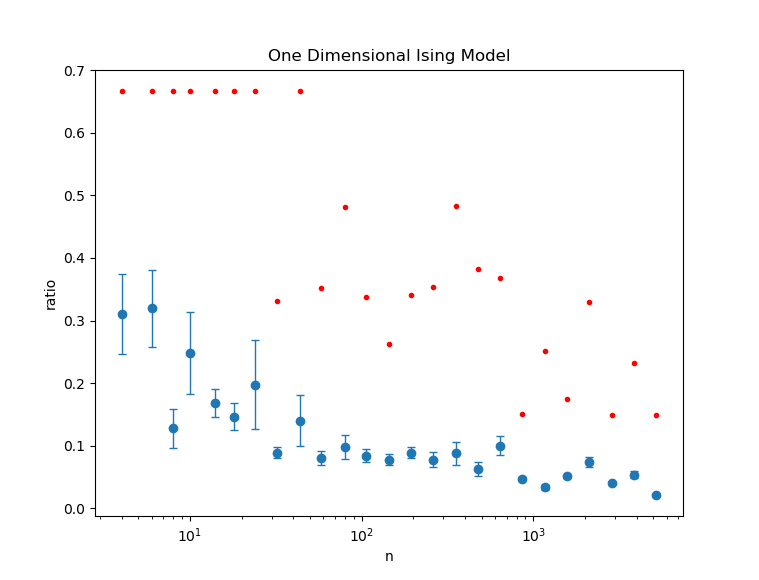
\includegraphics[width=0.9\textwidth]{avgchainplot(4,5200,2,20,25)}
	\label{fig:1}
\end{figure}

# $\lambda=\alpha/\beta$

\begin{figure}[H]
	\centering
	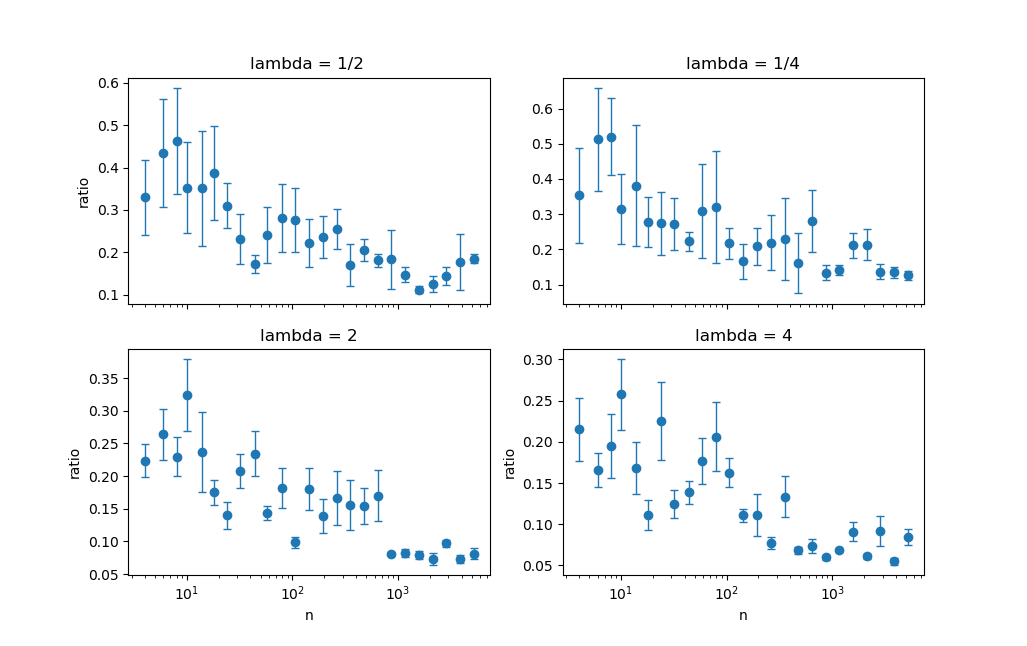
\includegraphics[width=1.1\textwidth]{tfiplots2}
	\label{fig:2}
\end{figure}

# $H =  X_1X_{2}+Z_1Z_{2}+X_{3}+X_{4}+X_5X_{6}+Z_5Z_{6}+X_{7}+X_{8}\ldots$

\begin{figure}[h]
	\centering
	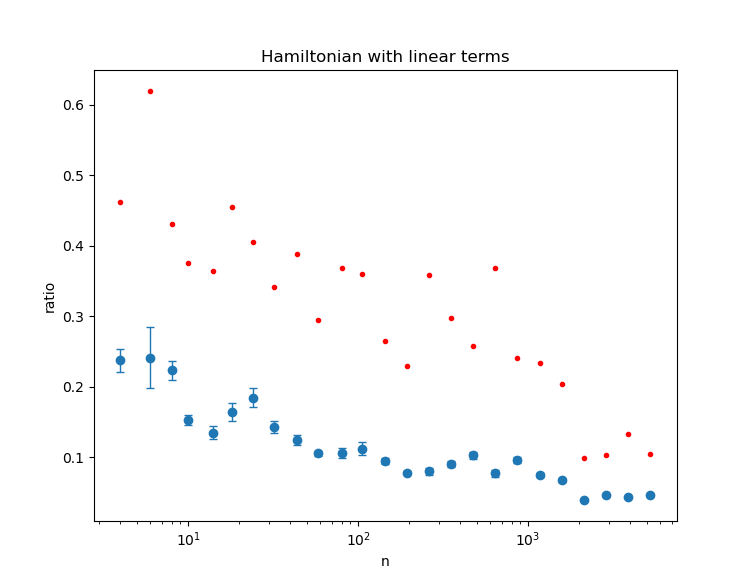
\includegraphics[width=0.9\textwidth]{avgplot(4,5200,2,20,25}
	\label{fig:3}
\end{figure}

# Next steps

+ Exactly solve the semidefinite program

+ Find optimal values for the constant $c$


# The qutrit Bloch-space

We represent a state $\rho$ with the help of a $d^2-1$-dimensional Bloch vector $\bm{\tau}$.
$$\rho = \frac{1}{d} \mathds{1} + \sum_{i=1}^{d^2-1} \tau_i \sigma_i$$

For $d\ge3$, there exist Bloch vectors with $\left|\tau\right|\le 1$ which do not correspond to a positive semi-definite matrix.

# Generalizing the Pauli matrices
The Gell-Mann matrices:
$$\lambda_1=\begin{pmatrix} 0 & 1 & 0 \\ 1 & 0 & 0 \\ 0 & 0 & 0 \end{pmatrix},
\lambda_2=\begin{pmatrix} 0 & -i & 0 \\ i & 0 & 0 \\ 0 & 0 & 0 \end{pmatrix},
\lambda_3=\begin{pmatrix} 1 & 0 & 0 \\ 0 & -1 & 0 \\ 0 & 0 & 0 \end{pmatrix},$$
$$\lambda_4=\begin{pmatrix} 0 & 0 & 1 \\ 0 & 0 & 0 \\ 1 & 0 & 0 \end{pmatrix},
\lambda_5=\begin{pmatrix} 0 & 0 & -i \\ 0 & 0 & 0 \\ i & 0 & 0 \end{pmatrix},
\lambda_6=\begin{pmatrix} 0 & 0 & 0 \\ 0 & 0 & 1 \\ 0 & 1 & 0 \end{pmatrix},$$
$$\lambda_7=\begin{pmatrix} 0 & 0 & 0 \\ 0 & 0 & -i \\ 0 & i & 0 \end{pmatrix},
\lambda_8=\frac{1}{\sqrt{3}} \begin{pmatrix} 1 & 0 & 0 \\ 0 & 1 & 0 \\ 0 & 0 & -2 \end{pmatrix}$$


# Generalizing the algorithm to qutrit systems

+ The Bloch space for qutrits has a solid sphere of radius $\frac{1}{2}$, i.e. all states corresponding to $\left| \bm{\tau} \right| \le \frac{1}{2}$ are valid states

+ Adapt the algorithm to this smaller sphere the cut-off then being $\frac{1}{2\sqrt{8}}$

+ $H=\sum_{i}\lambda_1^{i}\lambda_1^{i+1}$ with $\lambda^{n+1}_1=\lambda^{1}_1$

#

\begin{figure}[H]
	\centering
	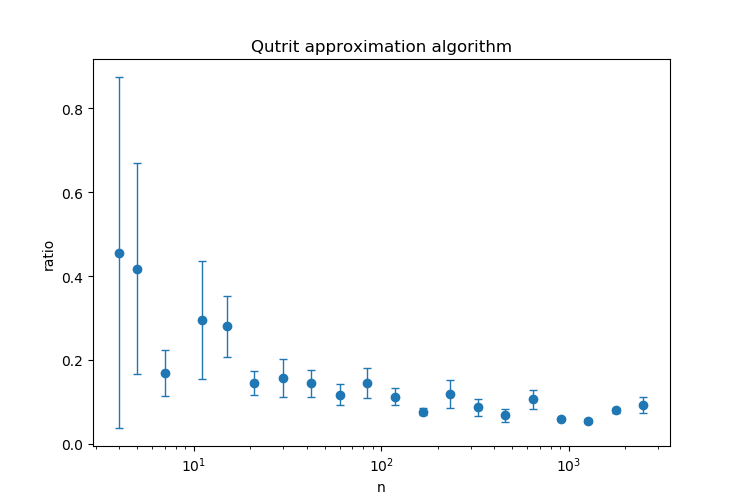
\includegraphics[width=0.8\textwidth]{tavgplot(4,2500,2,20,20).png}
	\label{fig:4}
\end{figure}

# Ideas for future work

+ Analytically investigate the effiency of this algorithm

+ Find more efficient rounding schemes that take into account the geometry of the Bloch space


#
